\chapter{Unfinished and future work}
\begin{figure}[H]
    \centering
    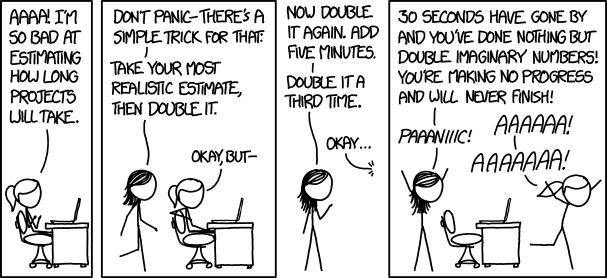
\includegraphics[width=\textwidth]{figures/estimating_time.png}
    \caption{Estimating Time \cite{xkcdEstimatingTime2016}}
    \label{fig:xkcd_time}
\end{figure}

\section{Introduction}


\section{Special stuff}
$\mathbf{SE_2(3)}$
More correct than $\mathbf{SE(3)}$ when working with an \gls{imu}

\section{Symforce}
Jinja used to call C++ from python automatically.

\section{Factor graph based smoothing}

\section{Uncertainties in the measurements}
Jabobians are easy to get using Symforce.

\section{Calibration}
